\documentclass[10pt,tikz,border=6pt]{standalone}
\usepackage[utf8]{inputenc}
\usepackage[T1]{fontenc}
\usepackage{amsmath}
\usetikzlibrary{arrows.meta,calc,decorations.pathreplacing,positioning}

\definecolor{syncblue}{RGB}{199,221,242}
\definecolor{headergray}{RGB}{224,224,224}
\definecolor{pilotgold}{RGB}{249,215,151}
\definecolor{datagreen}{RGB}{174,219,184}
\definecolor{tailviolet}{RGB}{218,204,232}

\begin{document}
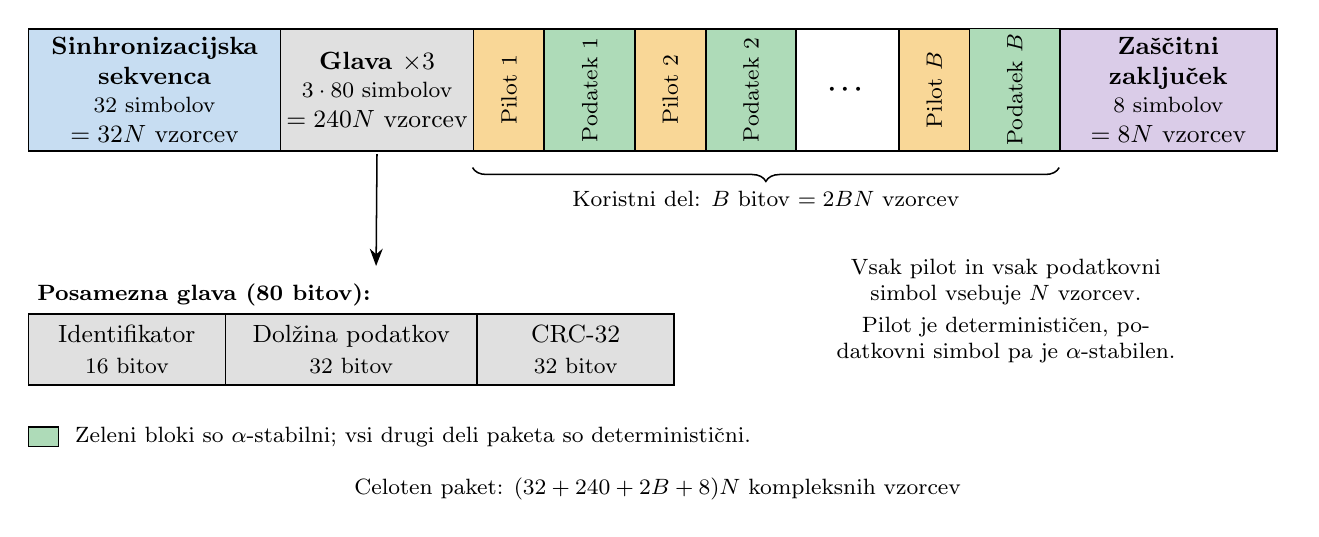
\begin{tikzpicture}[
  font=\small,
  packet/.style={draw=black, line width=0.65pt, minimum height=1.55cm,
                 align=center, inner sep=2pt},
  detail/.style={draw=black, line width=0.55pt, minimum height=0.9cm,
                 align=center, inner sep=2pt},
  note/.style={font=\footnotesize, align=center}
]

% Celoten oddajni paket
\node[packet, fill=syncblue, minimum width=3.20cm, anchor=south west]
  (sync) at (0,4.30) {\textbf{Sinhronizacijska}\\\textbf{sekvenca}\\[-1pt]
  \footnotesize 32 simbolov\\$=32N$ vzorcev};

\node[packet, fill=headergray, minimum width=2.45cm, anchor=south west]
  (header) at (3.20,4.30) {\textbf{Glava $\times 3$}\\[-1pt]
  \footnotesize $3\cdot80$ simbolov\\$=240N$ vzorcev};

\node[packet, fill=pilotgold, minimum width=0.90cm, anchor=south west]
  (p1) at (5.65,4.30) {\rotatebox{90}{\footnotesize Pilot 1}};
\node[packet, fill=datagreen, minimum width=1.15cm, anchor=south west]
  (d1) at (6.55,4.30) {\rotatebox{90}{\footnotesize Podatek 1}};
\node[packet, fill=pilotgold, minimum width=0.90cm, anchor=south west]
  (p2) at (7.70,4.30) {\rotatebox{90}{\footnotesize Pilot 2}};
\node[packet, fill=datagreen, minimum width=1.15cm, anchor=south west]
  (d2) at (8.60,4.30) {\rotatebox{90}{\footnotesize Podatek 2}};
\node[packet, fill=white, minimum width=1.30cm, anchor=south west]
  (dots) at (9.75,4.30) {$\boldsymbol{\cdots}$};
\node[packet, fill=pilotgold, minimum width=0.90cm, anchor=south west]
  (pb) at (11.05,4.30) {\rotatebox{90}{\footnotesize Pilot $B$}};
\node[packet, fill=datagreen, minimum width=1.15cm, anchor=south west]
  (db) at (11.95,4.30) {\rotatebox{90}{\footnotesize Podatek $B$}};

\node[packet, fill=tailviolet, minimum width=2.75cm, anchor=south west]
  (tail) at (13.10,4.30) {\textbf{Zaščitni}\\\textbf{zaključek}\\[-1pt]
  \footnotesize 8 simbolov\\$=8N$ vzorcev};

\draw[decorate, decoration={brace, amplitude=5pt, mirror}, line width=0.55pt]
  (5.65,4.10) -- node[note, below=5pt]
  {Koristni del: $B$ bitov $=2BN$ vzorcev} (13.10,4.10);

% Razčlenitev glave
\draw[-{Stealth[length=2.2mm]}, line width=0.55pt]
  ($(header.south)+(0,-0.03)$) -- (4.425,2.85);
\node[note, anchor=west] at (0,2.48) {\textbf{Posamezna glava (80 bitov):}};
\node[detail, fill=headergray, minimum width=2.50cm, anchor=north west]
  at (0,2.25) {Identifikator\\\footnotesize 16 bitov};
\node[detail, fill=headergray, minimum width=3.20cm, anchor=north west]
  at (2.50,2.25) {Dolžina podatkov\\\footnotesize 32 bitov};
\node[detail, fill=headergray, minimum width=2.50cm, anchor=north west]
  at (5.70,2.25) {CRC-32\\\footnotesize 32 bitov};

% Razlaga simbolov koristnega dela
\node[note, anchor=west, text width=7.0cm] at (8.80,2.28) {
  Vsak pilot in vsak podatkovni simbol vsebuje $N$ vzorcev.\\[2pt]
  Pilot je determinističen, podatkovni simbol pa je $\alpha$-stabilen.
};

% Skupni opombi
\node[draw, fill=datagreen, minimum width=0.38cm, minimum height=0.25cm]
  at (0.20,0.68) {};
\node[note, anchor=west] at (0.48,0.68)
  {Zeleni bloki so $\alpha$-stabilni; vsi drugi deli paketa so deterministični.};
\node[note] at (8.00,0.02)
  {Celoten paket: $(32+240+2B+8)N$ kompleksnih vzorcev};

\end{tikzpicture}
\end{document}
